% AnaTele — Technical report: architecture and mathematics
% Build: pdflatex AnaTele_Technical_Report.tex   (run twice for the table of contents)
\documentclass[11pt,a4paper]{article}

\usepackage[margin=2.3cm]{geometry}
\usepackage[T1]{fontenc}
\usepackage[utf8]{inputenc}
\usepackage{lmodern}
\usepackage{amsmath,amssymb}
\usepackage{booktabs}
\usepackage{tabularx}
\usepackage{xcolor}
\usepackage{enumitem}
\usepackage{listings}
\usepackage{tikz}
\usetikzlibrary{arrows.meta,positioning,fit,backgrounds}
\usepackage[colorlinks=true,linkcolor=blue!50!black,urlcolor=blue!50!black]{hyperref}

\definecolor{accent}{HTML}{E4572E}
\lstset{basicstyle=\ttfamily\small,columns=fullflexible,frame=single,framerule=0.3pt,
        breaklines=true,keepspaces=true,showstringspaces=false}
\newcommand{\code}[1]{\texttt{#1}}
\newcommand{\us}{\,\mu\text{s}}
\setlist{itemsep=2pt,topsep=4pt}
\setlength{\emergencystretch}{3em}
\sloppy

\title{\textbf{AnaTele}\\[4pt]\large Evidence-first investigation of ArduPilot flight logs\\[2pt]
\normalsize Architecture, mathematics and design decisions}
\author{Avinash\\\small \url{https://github.com/Avinashistoocool/AnaTele}}
\date{Version 0.4.0 \quad October 2026}

\begin{document}
\maketitle

\begin{abstract}
AnaTele is an open-source desktop tool that reads ArduPilot flight recordings (Mission Planner
\code{.tlog}, DataFlash \code{.bin}/\code{.log}, mapped \code{.csv}) and turns them into an
investigation: when the aircraft actually took off, what each subsystem was doing before the
event, which screening rules fire, and how the plausible causes rank against each other. Every
statement is linked to the exact log record that supports it. This report documents the
motivation, the system architecture, and all of the mathematics used: binary framing, clock
segmentation, signal normalisation, flight-phase inference, thrust-vector tracking error, motor
saturation and mixer decomposition, persistence and counter detectors, the hypothesis-ranking
score, waypoint geometry, plot down-sampling, 3D replay kinematics, the fault-injection flight
simulator, and the integrity model of the shareable \code{.ant} analysis format.
\end{abstract}

\tableofcontents
\newpage

%====================================================================
\section{Motivation}
%====================================================================

AnaTele started with a crash. While leading the NIDAR \emph{RescueSwarm} problem statement, our
team began offline flight testing with cameras and our own algorithms, and the aircraft went down
twice. Afterwards the investigation looked like this:

\begin{enumerate}
  \item Thousands of lines of telemetry, read by hand.
  \item A general-purpose AI assistant, which correctly pointed at the compass (it had not been
        calibrated properly, which is now part of our pre-flight checklist) but could say
        nothing else about the flight.
  \item Mission Planner's graphing, which was slow on long logs and whose heading display
        was confusing exactly when the yaw estimate was wrong.
\end{enumerate}

Reading the log manually showed that there was much more in it: the order of events before the
disarm, how the motors were being driven, whether vibration was a cause or only a consequence of
the impact, and which questions the log simply could not answer. AnaTele automates that reading.
It works out the flight phases, evaluates a versioned rule pack, ranks candidate causes using the
evidence for and against each one, plots the signals that matter, and replays where the aircraft
actually went.

\subsection{Design principles}
These rules come from the design document (\code{docs/DESIGN.md}) and apply everywhere in the code:

\begin{description}
  \item[Observation $\neq$ interpretation.] Decoded records are immutable evidence. Derived
        signals, findings and hypotheses are labelled as such and point back to record ids.
  \item[Missing is unknown, never healthy.] Every rule result is one of four states:
        \emph{triggered}, \emph{not triggered}, \emph{unassessable}, \emph{not applicable}.
        Absent data produces \emph{unassessable}, not a pass.
  \item[No invented probabilities.] Hypotheses are ordered by an explicit, inspectable screening
        score, never by a probability (Section~\ref{sec:hyp} explains why).
  \item[Read-only.] There is no live MAVLink link, no parameter write and no flight command.
  \item[Reproducible.] Engine, rule-pack and semantic-pack versions and SHA-256 hashes are stored
        with every result.
\end{description}

%====================================================================
\section{System architecture}
%====================================================================

\begin{figure}[h]
\centering
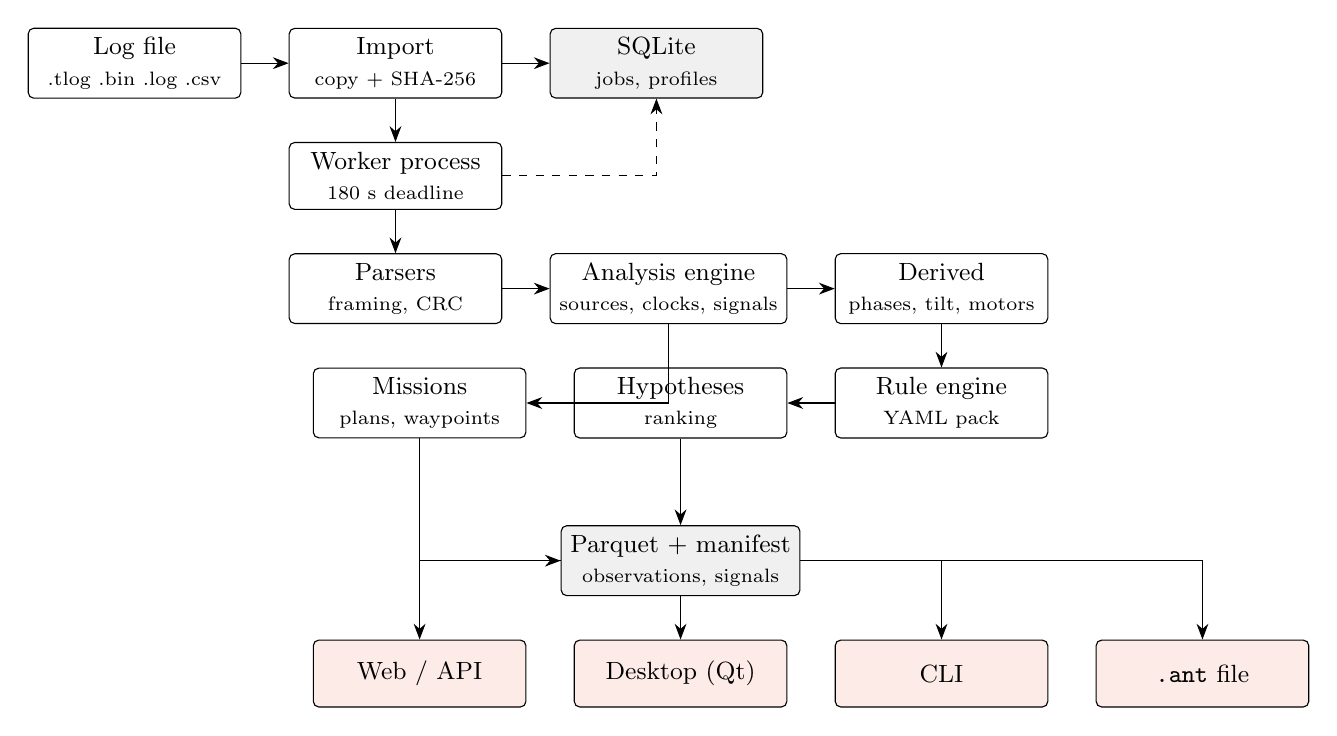
\begin{tikzpicture}[
  box/.style={draw,rounded corners=2pt,minimum width=2.7cm,minimum height=0.85cm,align=center,font=\small,fill=white},
  store/.style={box,fill=gray!12},
  ui/.style={box,fill=accent!12},
  >={Stealth[length=2mm]}, node distance=0.55cm and 0.6cm]
  \node[box] (file) {Log file\\\scriptsize .tlog .bin .log .csv};
  \node[box,right=of file] (import) {Import\\\scriptsize copy + SHA-256};
  \node[store,right=of import] (db) {SQLite\\\scriptsize jobs, profiles};
  \node[box,below=of import] (worker) {Worker process\\\scriptsize 180 s deadline};
  \node[box,below=of worker] (parse) {Parsers\\\scriptsize framing, CRC};
  \node[box,right=of parse] (engine) {Analysis engine\\\scriptsize sources, clocks, signals};
  \node[box,right=of engine] (derived) {Derived\\\scriptsize phases, tilt, motors};
  \node[box,below=of derived] (rules) {Rule engine\\\scriptsize YAML pack};
  \node[box,left=of rules] (hyp) {Hypotheses\\\scriptsize ranking};
  \node[box,left=of hyp] (missions) {Missions\\\scriptsize plans, waypoints};
  \node[store,below=1.1cm of hyp] (parquet) {Parquet + manifest\\\scriptsize observations, signals};
  \node[ui,below=of parquet] (desk) {Desktop (Qt)};
  \node[ui,left=of desk] (web) {Web / API};
  \node[ui,right=of desk] (cli) {CLI};
  \node[ui,right=of cli] (ant) {\code{.ant} file};
  \draw[->] (file) -- (import); \draw[->] (import) -- (db);
  \draw[->] (import) -- (worker); \draw[->] (worker) -- (parse);
  \draw[->] (parse) -- (engine); \draw[->] (engine) -- (derived);
  \draw[->] (derived) -- (rules); \draw[->] (rules) -- (hyp);
  \draw[->] (engine.south) |- (missions.east);
  \draw[->] (hyp) -- (parquet); \draw[->] (missions) |- (parquet);
  \draw[->] (parquet) -- (desk); \draw[->] (parquet) -| (web); \draw[->] (parquet) -| (cli);
  \draw[->] (parquet) -| (ant);
  \draw[->,dashed] (worker.east) -| (db.south);
\end{tikzpicture}
\caption{Data flow. Shaded boxes hold persistent state; orange boxes are user interfaces.}
\label{fig:arch}
\end{figure}

\subsection{Components}

\begin{tabularx}{\linewidth}{@{}lX@{}}
\toprule
Module & Responsibility \\
\midrule
\code{parsers.py} & File-only readers. Timestamped MAVLink framing with CRC validation and resync;
DataFlash via pymavlink \code{DFReader}; a strict CSV schema. Each record gets an id, byte offset
and length. \\
\code{analysis.py} & Streaming engine: source classification, clock epochs, arming episodes,
STATUSTEXT reassembly, events, parameter snapshots, signal extraction. Writes Parquet and the
manifest. \\
\code{derived.py} & In-memory time-series store, flight-phase inference, tilt tracking error,
motor mapping and saturation flags, mixer decomposition, window statistics. \\
\code{rules.py}, \code{rules/core.yaml} & Declarative rule pack (20 rules, 9 detector types) and
hypothesis ranking. YAML is loaded with \code{safe\_load}; rules cannot execute code. \\
\code{semantics.py}, \code{semantics/*.yaml} & Firmware-specific meaning (ArduCopter 4.7.2 tied
to its git hash), parameter decoding, volatile parameters. \\
\code{missions.py} & Mission upload/download transactions, plan versions, waypoint status. \\
\code{compare.py} & Parameter diff, phase-aligned flight comparison, per-aircraft trends. \\
\code{store.py}, \code{worker.py} & SQLite job queue, data directories, worker process with a
deadline. \\
\code{desktop.py}, \code{api.py}, \code{cli.py} & PySide6 + matplotlib desktop app, FastAPI web UI,
command line. \\
\code{replay.py} & 3D flight path and attitude glyph, PNG/GIF export. \\
\code{simulator.py} & Physics-based quadcopter with fault scenarios that writes real \code{.tlog}
files. \\
\code{antfile.py} & Shareable \code{.ant} analysis container: export, validation, import. \\
\bottomrule
\end{tabularx}

\subsection{Process and storage model}
Importing copies the file into \code{uploads/}, computes its SHA-256 and inserts a \emph{queued}
job row. A scheduler claims jobs with an \code{BEGIN IMMEDIATE} transaction (so two schedulers
can never claim the same job) and starts a \textbf{separate worker process}. A parser crash, a
memory blow-up or a pathological file can therefore not take down the UI, and the worker is
killed after $180$\,s. The worker streams records into two CSV spools, which are converted to
columnar \textbf{Parquet} files:

\begin{itemize}
  \item \code{observations.parquet}: one row per decoded record (time, clock, source, epoch,
        message, offset, length, sequence, quality, JSON payload). This is the evidence store.
  \item \code{signals.parquet}: normalised long-format samples $(id,t,epoch,source,name,value,unit)$
        including derived signals.
\end{itemize}

The manifest (findings, rule results, phases, missions, metrics, limitations, hashes) is stored as
JSON in the job row. Queries over Parquet use an embedded DuckDB with a 256\,MB memory limit and
two threads.

\subsection{Resource limits}
Upload 100\,MiB; $10^6$ records; 20\,000 events; $6\times10^6$ in-memory derived samples; 64\,KiB
maximum resync span; \code{.ant} file 1\,GiB. Each limit fails loudly; none silently truncates
evidence.

%====================================================================
\section{Ingestion mathematics}
%====================================================================

\subsection{Telemetry log framing}
A Mission Planner \code{.tlog} is a concatenation of
\[
\underbrace{t_{\text{UTC}}}_{8\text{ bytes, big-endian, }\mu s}\;\Vert\;\text{MAVLink frame}.
\]
For a frame with start marker $m$ and payload length $n$, the header length is $h=10$ for MAVLink 2
($m=\mathtt{0xFD}$) and $h=6$ for MAVLink 1 ($m=\mathtt{0xFE}$). With signing flag $s\in\{0,1\}$
the total frame length is
\[
L = h + n + 2 + 13s,
\]
where $2$ is the CRC and $13$ the signature. A candidate is accepted only if
\[
m\in\{\mathtt{0xFD},\mathtt{0xFE}\}\quad\wedge\quad
946\,684\,800\times10^{6} \le t_{\text{UTC}} \le 4\,102\,444\,800\times10^{6},
\]
i.e.\ the timestamp lies between 2000-01-01 and 2100-01-01, and if the CRC-16/MCRF4XX (X.25) over
the header and payload, seeded with the message's \code{CRC\_EXTRA}, matches. On failure the reader
advances one byte and retries (\emph{resync}). If more than $65\,536$ bytes pass without a valid
frame, recovery stops and the file is rejected rather than guessed at. Every resynchronised span,
truncated tail, unknown message id and unsupported incompatibility flag becomes a diagnostic with a
byte offset. Signed frames are kept and labelled \emph{signature unverified}.

\subsection{Clock epochs}
A log mixes clocks: the ground station's capture clock (UTC), the autopilot's
\code{time\_boot\_ms}, and DataFlash \code{TimeUS}. Reboots and capture glitches make them jump
backwards, and comparing samples across such a jump would be meaningless. AnaTele therefore assigns
each record an \emph{epoch}
\[
e = 10\,000\,c + b,
\]
where $c$ counts capture-clock regressions and $b$ counts per-source boot regressions:

\begin{align*}
c &\leftarrow c+1 && \text{if } t_{\text{capture}} < t_{\text{capture}}^{\text{prev}} - 2\text{ s},\\
b &\leftarrow b+1 && \text{if } \text{boot\_ms} < \text{boot\_ms}^{\text{prev}} - 10\,000
                    \text{ and not a wrap},\\
b &\leftarrow b+1 && \text{if } \text{TimeUS} < \text{TimeUS}^{\text{prev}} - 10^{6}\ \text{(DataFlash)}.
\end{align*}

A uint32 wrap is recognised when the previous value exceeds $\mathtt{0xF0000000}$ and the new one is
below $10^5$. All series, episodes and rules are keyed by \emph{(source, epoch)}; an open armed
episode crossing an epoch boundary is closed with the note ``clock discontinuity; end time unknown''.

\subsection{Source classification}
Each MAVLink \code{(system, component)} pair is a source. Its role comes from what it says, not
from its id:
\begin{itemize}
  \item a \code{HEARTBEAT} with \code{type = MAV\_TYPE\_GCS} $\Rightarrow$ ground station;
  \item a \code{HEARTBEAT} with a valid autopilot $\Rightarrow$ vehicle;
  \item \code{RADIO\_STATUS} from an unclassified source $\Rightarrow$ radio.
\end{itemize}
Only vehicle sources may arm. This prevents the classic mistake of reading the GCS heartbeat's
\code{base\_mode} as the aircraft's arming state. Armed state is
\[
\text{armed} = (\text{base\_mode} \mathbin{\&} \mathtt{MAV\_MODE\_FLAG\_SAFETY\_ARMED}) \ne 0,
\]
and each armed interval becomes an \emph{episode}.

\subsection{Signal normalisation}
Raw fields are converted to SI-like units with explicit scale factors, for example:
\[
\varphi_{\deg} = \tfrac{180}{\pi}\varphi_{\text{rad}},\quad
\text{lat}_{\deg} = 10^{-7}\,\text{lat}_{\text{int}},\quad
h_{\text{m}} = 10^{-3}\,h_{\text{mm}},\quad
V = 10^{-3}\,V_{\text{mV}},\quad I = 10^{-2}\,I_{\text{cA}}.
\]
Sentinels are treated as absence, not as measurements: a battery voltage of 0 or 65\,535 (no
monitor configured), current $-1$, RC values $0$ or $65\,535$, and non-finite floats are dropped.

\subsection{Parameter decoding}
\code{PARAM\_VALUE} transports every parameter as a 32-bit float, but integer parameters may be
encoded either by \emph{C-cast} ($\text{float}(v)$) or \emph{bytewise} (the integer's bytes
reinterpreted as a float). AnaTele uses the vehicle's \code{AUTOPILOT\_VERSION} capability bits, or
the firmware semantic pack, to choose. Under C-cast a value is accepted only if it is integral and
inside the declared type's range:
\[
\text{decode}(r,\tau)=
\begin{cases}
\lfloor r\rfloor & r\in\mathbb{Z},\ r\in[\ell_\tau,u_\tau]\\
\text{unverified} & \text{otherwise}
\end{cases}
\qquad
[\ell_\tau,u_\tau]\in\{[0,2^8\!-\!1],[-2^7,2^7\!-\!1],\dots,[-2^{31},2^{31}\!-\!1]\}.
\]
Under bytewise encoding the original 4 wire bytes (kept in the record) are unpacked little-endian
with the declared type. If both capability bits are set, the encoding is \emph{ambiguous} and the
value stays unverified, so rules that depend on it become \emph{unassessable}.

Snapshot completeness compares the observed indices $\mathcal{I}$ with the reported count $N$:
complete iff $|\{0,\dots,N-1\}\cap\mathcal{I}| = N$. Even then it is labelled ``not atomic''
because values arrive at different times.

%====================================================================
\section{Time-series store}
%====================================================================

Each $(source, epoch, name)$ owns three parallel typed arrays $t_i$ (int64\,$\mu$s), $v_i$ (float64)
and $r_i$ (record id), kept sorted by $t$. Out-of-order samples are inserted with binary search.
Range queries return the index interval
\[
[\,\text{lo},\text{hi}) = [\,\text{bisect\_left}(t,a),\ \text{bisect\_right}(t,b)\,)
\]
in $O(\log n)$. The \emph{nearest-sample} query used to pair signals is
\[
\text{nearest}(t^\ast,\delta)=\arg\min_{i\in\{k-1,k\}}|t_i-t^\ast|
\quad\text{subject to } |t_i-t^\ast|\le\delta,\qquad k=\text{bisect\_left}(t,t^\ast),
\]
returning nothing if no sample lies within $\delta$. AnaTele never interpolates evidence. Pairing
uses the nearest real sample or nothing.

%====================================================================
\section{Flight-phase inference}
%====================================================================

Rules must distinguish ``before the problem'' from ``during the crash'': vibration at impact is a
consequence, not a cause. Phases are therefore computed per armed episode $[t_a, t_d]$.

\paragraph{Reported.} If the vehicle sends \code{EXTENDED\_SYS\_STATE} with landed state \emph{In
air} or \emph{Taking off}, the first such time is the takeoff ($\text{status}=$
\emph{airborne\_reported}).

\paragraph{Inferred.} Otherwise, with home-relative altitude samples $h_i$:
\begin{align*}
\bar h &= \operatorname{median}\{h_i : t_a \le t_i \le t_a + 2\text{ s}\}
   && \text{(armed baseline)}\\
i_{\text{rise}} &= \min\{i : h_i - \bar h \ge 1.0\text{ m}\}
   && \text{(clear climb)}\\
\text{demand} &: \exists\, j:\ t_j\in[t_{\text{rise}}-5\text{ s},\,t_{\text{rise}}],\ 
   \text{throttle}_j \ge 10\% \ \vee\ u_{k,j}\ge 0.25
   && \text{(the motors were driving it)}\\
i_{\text{takeoff}} &= \max\{i < i_{\text{rise}} : h_i - \bar h \le 0.2\text{ m}\}
   && \text{(backtrack to lift-off)}
\end{align*}
where $u_{k,j}$ is motor $k$'s normalised output (Section~\ref{sec:motors}). No rise gives
\emph{no\_airborne\_evidence}. A rise without demand is treated as estimator drift. No altitude at
all gives \emph{unassessable}. The median baseline makes the estimate robust to a few noisy
barometer samples at arming.

\paragraph{Event markers.}
\begin{align*}
t_{\text{excursion}} &= \min\{t_i\ge t_{\text{takeoff}} : |\varphi_i|>60^\circ \vee |\theta_i|>60^\circ\},\\
t_{\text{pre-end}} &= \min\bigl(t_{\text{excursion}},\ t_{\text{crash}}-3\text{ s}\bigr),\\
t_{\text{air-end}} &= \min\bigl(t_{\text{excursion}},\ t_{\text{crash}}-3\text{ s},\ 
   \max\{t_i : h_i-\bar h\ge 0.5\},\ t_d\bigr).
\end{align*}
The 3\,s guard keeps the impact out of the \emph{pre-event} window. Rules then choose one of five
windows: \emph{airborne}, \emph{airborne\_pre\_event}
$=[t_{\text{takeoff}},t_{\text{pre-end}}]$, \emph{airborne\_with\_event}, \emph{event\_and\_after}
and \emph{armed\_pre\_takeoff}. All thresholds are recorded in the output, because they are
analysis choices, not firmware behaviour.

%====================================================================
\section{Thrust-vector (tilt) tracking error}
%====================================================================

A multirotor can only push along its body $z$ axis, so the meaningful control error is the angle
between where the controller wanted the thrust to point and where it actually pointed. For roll
$\varphi$ and pitch $\theta$ (ZYX Euler, yaw ignored because it does not tilt the thrust), the body
thrust axis expressed in a yaw-free level frame is
\[
\hat{\mathbf z}(\varphi,\theta)=
\begin{pmatrix}\sin\theta\cos\varphi\\ -\sin\varphi\\ \cos\theta\cos\varphi\end{pmatrix},
\qquad \|\hat{\mathbf z}\|=1.
\]
The tracking error between desired $(\varphi_d,\theta_d)$ and estimated $(\varphi,\theta)$ is the
great-circle angle
\[
\boxed{\;\varepsilon = \arccos\bigl(\operatorname{clip}_{[-1,1]}\,
\hat{\mathbf z}(\varphi_d,\theta_d)\cdot\hat{\mathbf z}(\varphi,\theta)\bigr)\;}
\]
Unlike $|\varphi_d-\varphi|+|\theta_d-\theta|$, this is frame-independent and does not
double-count combined roll and pitch errors. ArduPilot's own crash check uses the same idea (an
angle error above $30^\circ$ for 2\,s).

\paragraph{Sources of the desired attitude.} \code{NAV\_CONTROLLER\_OUTPUT}
(\code{nav\_roll}, \code{nav\_pitch}), \code{ATTITUDE\_TARGET} or DataFlash \code{ATT.DesRoll}. The
first one seen is locked per source so that two definitions are never mixed. A quaternion target
$q=(w,x,y,z)$ is converted with
\[
\varphi=\operatorname{atan2}\!\bigl(2(wx+yz),\,1-2(x^2+y^2)\bigr),\qquad
\theta=\arcsin\!\bigl(\operatorname{clip}(2(wy-zx))\bigr).
\]

\paragraph{Pairing.} For each desired-roll sample at $t$, desired pitch must lie within 1\,ms and
estimated roll/pitch within 250\,ms (\code{nearest}). Otherwise no error sample is produced. The
limitation that desired and estimated values are sampled at different instants is reported in the
output.

%====================================================================
\section{Motors: saturation and mixer decomposition}\label{sec:motors}
%====================================================================

\subsection{Mapping}
Motors are found from \code{SERVO$n$\_FUNCTION} $\in\{33,\dots,40\}$ (motor $1\dots8$). With PWM
range $[P_{\min},P_{\max}]$ (\code{MOT\_PWM\_*}, falling back to \code{RC3\_*}) and spin limits
$s_{\min},s_{\max}$ (\code{MOT\_SPIN\_*}):
\[
\Delta P=P_{\max}-P_{\min},\qquad
P_{\text{floor}}=P_{\min}+s_{\min}\Delta P,\qquad
P_{\text{ceil}}=P_{\min}+s_{\max}\Delta P .
\]
For each output sample $P_k$ the normalised command and saturation flags are
\[
u_k=\frac{P_k-P_{\min}}{\Delta P},\qquad
F^{\text{floor}}_k=[P_k\le P_{\text{floor}}+2],\qquad
F^{\text{ceil}}_k=[P_k\ge P_{\text{ceil}}-2],
\]
with a $\pm2\,\mu$s tolerance for PWM quantisation. Samples where all outputs are at or below
$P_{\min}+1$ (disarmed or stopped) are skipped so that idle is not mistaken for saturation. If any
of these parameters is unknown, the motor rules are \emph{unassessable} and say why.

\subsection{Mixer decomposition}
Each motor $k$ has a geometry vector $(x_k,y_k,\sigma_k)$: $x$ = right ($\pm1$), $y$ = forward
($\pm1$), $\sigma=+1$ for counter-clockwise props. For QUAD/X:
\[
1:(+1,+1,+1),\quad 2:(-1,-1,+1),\quad 3:(-1,+1,-1),\quad 4:(+1,-1,-1).
\]
The share of the commands that goes into each axis is the normalised weighted sum
\[
D_{\text{roll}}=\frac{\sum_k x_k c_k}{\sum_k|x_k|},\qquad
D_{\text{pitch}}=\frac{\sum_k y_k c_k}{\sum_k|y_k|},\qquad
D_{\text{yaw}}=\frac{\sum_k \sigma_k c_k}{\sum_k|\sigma_k|},
\]
where $c_k$ is the PWM (time series) or the mean $\bar u_k$ (rule). $D_{\text{roll}}>0$ means the
right side works harder (the frame is being held up on the right), and $D_{\text{yaw}}>0$ means the
CCW propellers work harder.

\subsection{Imbalance rule}
Over the pre-event window (first 2\,s trimmed to exclude the spool-up),
\[
\bar u_k=\frac1{n_k}\sum_i u_{k,i},\qquad
\text{spread}=\max_k\bar u_k-\min_k\bar u_k,\qquad
\text{triggered}\iff\text{spread}>0.12 .
\]
If $|D_{\text{yaw}}|>2\max(|D_{\text{roll}}|,|D_{\text{pitch}}|)$, the report says that the
imbalance is predominantly yaw (one prop direction working harder). This points to twisted
mounts, a prop or direction mismatch, or sustained yaw demand, rather than a single weak motor.
A single weak motor shows up instead as roll and pitch imbalance towards that corner.

%====================================================================
\section{Rule engine}
%====================================================================

Rules are YAML data with an id, an integer version, a severity, a scope (\emph{event, source,
episode, series, snapshot}), a detector type and text templates. The whole pack is hashed with
SHA-256. The detectors are below.

\subsection{Persistence (vibration, tracking error, EKF ratio, saturation)}
Given samples $(t_i,v_i)$ in the windows $W$, a threshold $L$, a maximum gap $g$ and a duration
$T$, a \emph{run} is a maximal sequence of consecutive samples with
\[
v_i>L\quad\text{and}\quad t_{i}-t_{i-1}\le g .
\]
Its duration is $d=t_{\text{last}}-t_{\text{first}}$. The rule triggers if
\[
\max_{\text{runs}} d \ \ge\ T .
\]
A gap larger than $g$ breaks the run, so a dropout cannot be counted as ``still above''.
The core criteria are as follows.

\begin{center}
\begin{tabular}{@{}lll@{}}
\toprule
Rule & Signal & Criterion \\
\midrule
vibration-persistent-pre-event & \code{imu.*.vibration.*} & $>30$ m/s$^2$ for 2\,s, or $>60$ for 1\,s \\
tracking-loss & tilt error $\varepsilon$ & $>30^\circ$ for 0.5\,s \\
ekf-compass-innovation-pre-event & \code{ekf.*compass\_ratio} & $>1.0$ for 2\,s \\
motor-ceiling-saturation & $F^{\text{ceil}}_k$ & $>0.5$ for 1\,s \\
motor-floor-saturation-pre-event & $F^{\text{floor}}_k$ & $>0.5$ for 2\,s \\
\bottomrule
\end{tabular}
\end{center}

The vibration threshold can come from the aircraft profile. An EKF test ratio above 1 means
that the innovation exceeded its gate (the measurement disagreed with the prediction by more than
the filter's tolerance).

\paragraph{Resolution check (Nyquist-style).} If no run qualifies, absence is only informative
when the sampling can resolve the criterion. With the median sample interval $\widetilde{\Delta t}$,
\[
\widetilde{\Delta t}\ \ge\ T\ \text{for every criterion}\ \Longrightarrow\ \text{unassessable},
\]
because a 2\,s event cannot be ruled out by 2\,s-spaced samples. If only some criteria are
unresolvable, the result is \emph{not triggered} and the text names the unresolved ones. Fewer than
three samples in the window also gives \emph{unassessable}.

\subsection{Counter increments (accelerometer clipping)}
Clip counters are cumulative. For consecutive pairs with $t_{i+1}-t_i\le3$\,s,
\[
\Delta_i=v_{i+1}-v_i,\qquad
\text{added}=\sum_i\max(0,\Delta_i),\qquad
\text{resets}=|\{i:\Delta_i<0\}| .
\]
Negative steps (reboot or reset) are excluded rather than subtracted. The increment is reported
separately for the pre-event window and the event and after, so ``clipping at impact'' is not
confused with ``clipping in flight''.

\subsection{Event presence and sequence}
\emph{Presence} matches event kinds or a regular expression on reassembled STATUSTEXT. If the
source never recorded any text, the result is \emph{unassessable}, not \emph{not triggered}.
Optional context signals report the range within $\pm w$ seconds and compare it with a parameter
(for example, mapped throttle versus \code{FS\_THR\_VALUE}).

\emph{Sequence} looks for a precursor $p$ before an anchor $a$ (crash-check disarm):
\[
0\le t_a-t_p\le 20\text{ s}.
\]
It then adds \emph{support} if the EKF compass ratio was $>1$ for $\ge2$\,s in the 30\,s before
$p$, and a \emph{contradiction} if tilt error was already $>30^\circ$ for $\ge0.5$\,s before $p$
(the aircraft was already out of control, so the compass switch is more likely recovery than cause).

\subsection{Peak, coverage and parameter detectors}
\emph{Peak}: $\max_i v_i > L$ with the argmax record as evidence. \emph{Coverage}: triggers when no
battery signal exists during any armed episode (``power cannot be assessed''). \emph{Parameter}:
equality or bit test $\lfloor v\rfloor \mathbin{\&} 2^b\ne0$, only for verified values and, for
bit meanings, only under the matching firmware semantics. \emph{Profile}: $|v_{\text{obs}}-v_{\text{exp}}|
>10^{-4}$ for each declared expected parameter.

%====================================================================
\section{Hypothesis ranking}\label{sec:hyp}
%====================================================================

For each episode with a crash-check report, every hypothesis $H$ (estimator/magnetic,
thrust/configuration, vibration, power) declares supporting rules $r$, each with an evidence
\emph{family} $f(r)$ and a weight $w_r$, plus contradicting conditions with penalties $\pi_c$.
\[
\boxed{\;
S(H)=\sum_{f}\min\!\Bigl(C,\ \sum_{\substack{r\in H,\ f(r)=f\\ r\ \text{triggered}}} w_r\Bigr)
\;-\;\sum_{c\in H,\ c\ \text{holds}}\pi_c,\qquad C=1.5 .\;}
\]
The family cap $C$ stops correlated evidence from inflating the score. Ten reports from the same
saturated motor are one piece of propulsion evidence, not ten. The labels are as follows.

\begin{center}
\begin{tabularx}{\linewidth}{@{}Xl@{}}
\toprule
Condition & Label \\
\midrule
blocked (e.g.\ no power monitoring), or nothing assessed and nothing against & unassessable \\
support and contradictions both present & mixed support \\
$S\ge2$ & strong support \\
$1\le S<2$ & some support \\
$0<S<1$ & weak support \\
otherwise & limited or contradicting evidence \\
\bottomrule
\end{tabularx}
\end{center}

Hypotheses are sorted by (unassessable last, $-S$). For example, thrust/configuration:
\[
S=\min(1.5,\,1_{\text{tracking}})+\min(1.5,\,1_{\text{floor}}+0.75_{\text{imbalance}}+0.5_{\text{ceiling}}).
\]
With tracking loss, ceiling saturation and imbalance this gives $1+1.25=2.25$, which is
\emph{strong support}.

\paragraph{Why not a probability?} A posterior $P(H\mid E)$ needs priors (base rates of each failure
for this airframe) and likelihoods $P(E\mid H)$ that account for strong dependence between
signals. Neither exists for a single hobby or competition aircraft. Printing ``73\,\%'' would imply
calibration that the data cannot support. The score is an expert-weighted \emph{screening order}:
transparent, reproducible, and shown together with what supports it, what contradicts it, and
which measurement would discriminate (``\emph{ESC RPM telemetry and a motor-order test}'').

%====================================================================
\section{Missions and waypoint geometry}
%====================================================================

\subsection{Transactions and plan versions}
Upload (\code{MISSION\_COUNT}$\to$\code{REQUEST}$\to$\code{ITEM}$\to$\code{ACK}), download, partial
write and clear are reconstructed per (GCS, vehicle, mission type, epoch). Retransmissions,
restarts, conflicting items and broadcast ACKs are handled. Only an accepted transfer in which every
item was observed creates a plan version with high confidence. Otherwise the plan is marked
uncertain.

\subsection{Distance}
The horizontal distance between a recorded position and a waypoint uses the haversine formula with
the IUGG mean Earth radius $R=6\,371\,008.8$\,m:
\[
a=\sin^2\!\tfrac{\Delta\phi}{2}+\cos\phi_1\cos\phi_2\sin^2\!\tfrac{\Delta\lambda}{2},\qquad
d=2R\arcsin\!\bigl(\min(1,\sqrt a)\bigr).
\]

\subsection{Waypoint status}
For each item, let $d^\ast=\min_i d(p_i,w)$ over the episode's recorded positions, $r$ the acceptance
radius (\code{WP\_RADIUS\_M}, or \code{WPNAV\_RADIUS}/100), and $\sigma_h$ the GPS horizontal accuracy
at that instant:
\[
\text{status}=
\begin{cases}
\text{reported\_complete} & \code{MISSION\_ITEM\_REACHED}(seq)\ \text{observed}\\
\text{geometry\_consistent\_with\_completion} & d^\ast\le r+\sigma_h\\
\text{not\_visited\_in\_observed\_trajectory} & d^\ast> r+\sigma_h\ \wedge\ \max\Delta t_{\text{pos}}\le5\text{ s}\\
\text{completion\_not\_observed} & \text{otherwise (coverage gaps)}\\
\text{unassessable} & \text{no position or no target}
\end{cases}
\]
The coverage condition matters: ``not visited'' is only claimed when there is no gap longer than
5\,s in which the aircraft could have passed the waypoint unrecorded. No interpolation is performed.

%====================================================================
\section{Statistics, comparison and plotting}
%====================================================================

\paragraph{Window statistics.} For values $v_{(1)}\le\dots\le v_{(n)}$ in a window: $n$, mean, min,
max and $p_{95}=v_{(\min(n,\lfloor0.95n\rfloor+1))}$ (nearest-rank). These feed the Flight Statistics
grid, the comparison table and the trends.

\paragraph{Comparison and trends.} Two flights are aligned by \emph{phase}, not by clock: metrics
are computed over each one's own pre-event airborne window. Parameter diffs ignore volatile
parameters and use a relative tolerance $|a-b|>10^{-6}\max(1,|a|)$. Trends group flights by the
profile's aircraft key and plot each metric in chronological order.

\paragraph{Plot down-sampling.} Sending $10^6$ points to a chart is wasteful, and naive decimation
hides spikes. The API keeps both extremes per bucket. For $n$ samples in an epoch and a budget of
$M$ points,
\[
B=\max\!\bigl(1,\lceil n/(M/2)\rceil\bigr),\qquad
\text{bucket}(i)=\Bigl\lfloor\frac{i-1}{B}\Bigr\rfloor,
\]
and for each bucket it returns $\arg\min v$ and $\arg\max v$. Every spike survives in the plot.
This envelope is used only for display and is never used for diagnosis.

%====================================================================
\section{3D replay}
%====================================================================

Positions are projected to a local tangent plane around the first fix $(\phi_0,\lambda_0)$ with the
equirectangular approximation (error well below GPS noise over a few kilometres):
\[
N=(\phi-\phi_0)\cdot111\,320,\qquad
E=(\lambda-\lambda_0)\cdot111\,320\cos\phi_0,\qquad U=h_{\text{home}} .
\]
Because the coordinates are local metres, screenshots do not reveal the flying field.
The aircraft glyph is drawn by rotating body-frame arm vectors (forward--right--down) to NED with
\[
R_{\text{NED}\leftarrow\text{FRD}}=
\begin{pmatrix}
c_\psi c_\theta & c_\psi s_\theta s_\varphi-s_\psi c_\varphi & \cdot\\
s_\psi c_\theta & s_\psi s_\theta s_\varphi+c_\psi c_\varphi & \cdot\\
-s_\theta & c_\theta s_\varphi & \cdot
\end{pmatrix},
\]
using only the first two columns because arms lie in the body $xy$ plane, and then converting to ENU
$(E,N,-D)$ for plotting. The path is coloured by flight mode, with markers for takeoff, attitude
excursion, crash report and waypoint status.

%====================================================================
\section{Flight simulator}
%====================================================================

The simulator exists to test the analyser against ground truth. It produces byte-exact
\code{.tlog} captures using the real MAVLink encoder, so every parser, rule and plot runs on it
unchanged. It is deterministic for a given seed.

\subsection{Airframe}
Mass $m=1.6$\,kg, arm $a=0.18$\,m, inertia $I=(0.022,0.022,0.04)$\,kg\,m$^2$, hover throttle
$h=0.38$, yaw coefficient $k=0.016$, linear drag $c_d=0.35$. Maximum thrust per motor follows
from hover:
\[
T_{\max}=\frac{mg}{4h},\qquad \ell=a\cdot\tfrac{\sqrt2}{2}\ \text{(lever arm on X frame)}.
\]

\subsection{Guidance}
Toward target $(n_t,e_t,u_t)$ at distance $D$:
\[
v_{\text{des}}=\min(5,\,0.8D)\frac{(\Delta n,\Delta e)}{D},\qquad
v_{u,\text{des}}=\operatorname{clip}\bigl(1.2(u_t-u),\,-1.5,\,2\bigr),\qquad
\psi_{\text{des}}=\operatorname{atan2}(\Delta e,\Delta n).
\]
A waypoint is reached when the horizontal distance is at most 2\,m and the vertical distance below 2\,m. RTL climbs to at
least 10\,m, returns and switches to LAND within 2\,m of home.

\subsection{Attitude and thrust control}
Velocity error becomes acceleration demand $a_{n,e}=\operatorname{clip}(1.4(v_{\text{des}}-v),\pm4)$,
rotated into the \emph{estimated} heading $\hat\psi=\psi+\psi_{\text{err}}$ (this is how a compass
error corrupts the flight):
\[
a_{\text{fwd}}=a_n\cos\hat\psi+a_e\sin\hat\psi,\qquad
a_{\text{right}}=-a_n\sin\hat\psi+a_e\cos\hat\psi,
\]
\[
\theta_d=\operatorname{clip}\!\bigl(-\operatorname{atan2}(a_{\text{fwd}},g),\pm0.52\bigr),\qquad
\varphi_d=\operatorname{clip}\!\bigl(\operatorname{atan2}(a_{\text{right}},g),\pm0.52\bigr).
\]
Collective thrust compensates tilt:
\[
\tau_c=\frac{m\,(g+a_u)}{\max(0.3,\cos\varphi\cos\theta)\cdot4T_{\max}},\qquad
a_u=\operatorname{clip}\bigl(2.5(v_{u,\text{des}}-v_u),-4,5\bigr).
\]
PD attitude torques:
\[
\tau_\varphi=I_x\bigl(100(\varphi_d-\varphi)-16p\bigr),\quad
\tau_\theta=I_y\bigl(100(\theta_d-\theta)-16q\bigr),\quad
\tau_\psi=I_z\bigl(9\,\mathrm{wrap}(\psi_d-\hat\psi)-6r\bigr).
\]

\subsection{Mixer with ArduPilot-style priority}
Per-motor roll/pitch and yaw contributions:
\[
\rho_k=\frac{-x_k\tau_\varphi+y_k\tau_\theta}{4\ell T_{\max}},\qquad
\gamma_k=\frac{\sigma_k\tau_\psi}{4kT_{\max}} .
\]
With limits $[s_{\min},s_{\max}]=[0.15,0.95]$:
\begin{enumerate}
  \item Roll/pitch first: if $\max\rho-\min\rho>s_{\max}-s_{\min}$, scale $\rho$ to fit.
  \item Shift the collective so that $\tau_c+\rho_k$ fits the range:
        $\delta=\max(0,\max_k(\tau_c+\rho_k)-s_{\max})-\max(0,s_{\min}-\min_k(\tau_c+\rho_k))$,
        $b_k=\tau_c-\delta+\rho_k$.
  \item Yaw last, scaled by the remaining headroom:
        $\eta=\min_k\min(s_{\max}-b_k,\,b_k-s_{\min})$,
        $u_k=\operatorname{clip}\bigl(b_k+\operatorname{clip}(\eta/\max|\gamma|,0,1)\gamma_k\bigr)$.
\end{enumerate}
This reproduces the real failure signature: when a motor weakens, yaw authority goes first,
then roll/pitch saturate, then the attitude diverges.

\subsection{Rigid-body dynamics}
Motor forces $F_k=h_kT_{\max}u_k$ with health $h_k\in[0,1]$ give
\[
\tau_\varphi=-\ell\sum_kx_kF_k,\quad
\tau_\theta=\ell\sum_ky_kF_k,\quad
\tau_\psi=k\sum_k\sigma_kF_k,
\]
\[
\dot p=\tau_\varphi/I_x-0.5p,\quad \dot q=\tau_\theta/I_y-0.5q,\quad \dot r=\tau_\psi/I_z-0.8r .
\]
Translational acceleration from total thrust $A=\sum F_k/m$, rotated by attitude and with drag
relative to the wind $\mathbf w(t)=(w_n+0.6\sin(t/7),\,w_e)$:
\[
a_{\text{fwd}}=-A\sin\theta\cos\varphi,\quad a_{\text{right}}=A\sin\varphi,\quad
a_{\text{up}}=A\cos\theta\cos\varphi-g,
\]
\[
\dot v_n=a_{\text{fwd}}\cos\psi-a_{\text{right}}\sin\psi-c_d(v_n-w_n),\quad
\dot v_e=a_{\text{fwd}}\sin\psi+a_{\text{right}}\cos\psi-c_d(v_e-w_e),\quad
\dot v_u=a_{\text{up}}-c_dv_u .
\]
Integration is explicit Euler with $\Delta t=10$\,ms. Ground contact zeroes velocity, and an
impact faster than 2.5\,m/s is recorded.

\subsection{Crash check}
As in ArduCopter, in AUTO/RTL/LAND/LOITER the thrust-axis angle error $\varepsilon$ is computed
from the desired and actual attitude. If $\varepsilon>30^\circ$ for 2\,s, the simulator emits
\code{Crash: Disarming: AngErr=\ldots} and disarms.

\subsection{Fault models}
\begin{tabularx}{\linewidth}{@{}lX@{}}
\toprule
Scenario & Model \\
\midrule
\code{motor\_failure} & Two seconds after WP2, motor 3 degrades linearly:
$h_3(t)=\max\bigl(0.3,\,1-0.06(t-t_f)\bigr)$. \\
\code{compass\_interference} & Innovation ratio grows with throttle $\bar u$:
$\rho_c=0.04+6\max(0,\bar u-0.2)$. The heading error integrates
$\dot\psi_{\text{err}}\propto\max(0,\bar u-0.25)$, clipped to $\pm1.4$\,rad, so the aircraft
toilet-bowls. After 4\,s above 1 the EKF switches compass (error $\times0.6$). After 25\,s it
triggers an EKF failsafe and LAND. \\
\code{vibration} & Vibration level $38+12\sin(t/3)+\mathcal N(0,3)$\,m/s$^2$ on the $z$ axis,
random clip increments, and torque noise $\mathcal N(0,0.01)$\,N\,m. \\
\code{radio\_failsafe} & PreArm radio warnings. In flight after WP2 the RC channels drop to zero,
followed by \emph{Radio Failsafe} and RTL. \\
\bottomrule
\end{tabularx}

\noindent Battery: open-circuit voltage decreases by coulomb counting,
$V_{oc}\mathrel{-}=I\,\Delta t/3600\cdot0.9$, and the terminal voltage is $V=V_{oc}-0.025I$ with
$I=1.5+32\bar u$\,A. Logs are labelled \code{SIMULATED FLIGHT} and located at the public SITL field.

\subsection{Validation}
The test suite asserts the expected outcome of each scenario:
\begin{itemize}
  \item \emph{nominal}: no critical findings and every waypoint \emph{reported\_complete};
  \item \emph{motor\_failure}: tracking loss, ceiling saturation and imbalance, with
        thrust/configuration ranked first;
  \item \emph{compass\_interference}: EKF ratio above 1 and a compass-selection event;
  \item \emph{vibration}: persistent vibration and pre-event clipping.
\end{itemize}
A private regression capture of a real crash (ArduCopter 4.7.2, two AUTO crash-check disarms) is
pinned by a JSON fixture.

%====================================================================
\section{The \texorpdfstring{\code{.ant}}{.ant} analysis format}
%====================================================================

An \code{.ant} (\emph{ANalysed Telemetry}) file is a finished, shareable analysis: a ZIP container,
following the same convention as ODF and EPUB.

\begin{center}
\begin{tabularx}{\linewidth}{@{}lX@{}}
\toprule
Entry & Contents \\
\midrule
\code{mimetype} & \code{application/vnd.anatele.analysis+zip}; first entry, stored uncompressed \\
\code{meta.json} & format version, versions, original file hash, profile, per-entry SHA-256 \\
\code{manifest.json} & the complete analysis \\
\code{observations.parquet} & decoded records (evidence) \\
\code{signals.parquet} & normalised and derived signals \\
\code{report.html} & printable report, readable without AnaTele \\
\code{original.<ext>} & optional; the untouched source log \\
\bottomrule
\end{tabularx}
\end{center}

\paragraph{Integrity.} For each entry $x$, \code{meta.json} stores $H(x)=\mathrm{SHA\text{-}256}(x)$,
and the original log is bound by the hash that was computed at import. On opening, every entry is
re-hashed while it is streamed and the file is rejected if $H'(x)\ne H(x)$. This detects accidental
corruption and naive edits. It is \emph{not} a signature, so it does not prove who created the file.

\paragraph{Untrusted-input handling.} Only whitelisted entry names are accepted, so path traversal
is impossible. Duplicate and encrypted entries are rejected, and only stored or deflate compression
is allowed. Sizes are capped \emph{during} decompression (which defeats zip bombs):
1\,GiB per file, 768\,MiB per Parquet, 1.5\,GiB in total. JSON structure and the Parquet column
schema are validated, and everything is extracted to a staging directory that is renamed into place
atomically or deleted. Nothing in the file is executed.

\paragraph{Privacy.} Without the original log the recipient still sees decoded records and the
flight path, but no raw bytes and no re-analysis. Both variants contain GPS positions, and the UI
says so before saving.

%====================================================================
\section{Security and distribution}
%====================================================================

\begin{itemize}
  \item The web UI binds to \code{127.0.0.1} and has a Host allow-list. It rejects cross-origin
        writes and sends \code{nosniff}, \code{DENY} framing and \code{no-referrer} headers. All
        dynamic HTML is escaped.
  \item The worker runs as a separate process with time and size limits. It is isolation, not a
        sandbox.
  \item Releases are built on GitHub Actions with SHA-pinned actions and read-only build jobs. Only
        a separate publish job holds write and attestation permissions. Runtime dependencies are
        installed from a hash-locked requirements file (\code{--require-hashes}). Release assets
        come with \code{SHA256SUMS.txt} and signed SLSA build-provenance attestations.
\end{itemize}

%====================================================================
\section{Interfaces}
%====================================================================

\begin{description}
  \item[Desktop.] A PySide6 window in the style of openMotor:
        \begin{itemize}
          \item left: recordings, profile and episodes;
          \item centre: stacked matplotlib plots with event and phase markers;
          \item right: X/Y axis signal selection;
          \item bottom: findings, hypotheses, rules, events, parameters, missions, flight path,
                evidence and statistics.
        \end{itemize}
        Clicking any plotted point opens the exact record (decoded payload and raw bytes).
  \item[Web/API.] FastAPI with the same analysis. Endpoints cover logs, events, rules, parameters,
        parameter diffs, series, positions, records, reports, \code{.ant} export and import,
        comparison and trends.
  \item[CLI.] \code{anatele [web|simulate|replay|analyse|export]}.
\end{description}

%====================================================================
\section{Limitations}
%====================================================================

\begin{itemize}
  \item Telemetry contains only what was streamed or recorded. Absence is never a healthy result.
  \item There are no calibrated probabilities, no per-core EKF innovation analysis from link
        telemetry, and no direct motor-failure diagnosis. Motor commands are not measured thrust.
  \item Phase inference without landed-state messages is heuristic and labelled as such.
  \item Clock segmentation is conservative. Capture time is not sensor time.
  \item Positions are estimates, and waypoint proximity is not proof of completion.
  \item The simulator is deliberately simple and proves nothing about a real aircraft.
\end{itemize}

%====================================================================
\section{Results and outlook}
%====================================================================

\subsection{Our crash log}
The capture is 2.2\,MB and contains 53\,465 records from ArduCopter 4.7.2 (\code{fb773567}). It has
no battery monitor and no landed-state messages. AnaTele found the following:

\begin{itemize}
  \item \textbf{Sources.} It separated the vehicle (1:1), the ground station (255:190) and the
        radio (51:68). It also decoded 973 parameters using the C-cast encoding of the semantic
        pack.
  \item \textbf{Episodes.} There were three armed episodes. In two of them the aircraft flew:
        takeoff was \emph{inferred} at about 640\,s and 980\,s, and each flight ended in a
        crash-check disarm (\code{AngErr=160>30}) about 17--20\,s after takeoff, just after
        mission item 2 had started. The third episode showed no airborne evidence.
  \item \textbf{Compass and EKF.} The EKF compass test ratio rose from about 0.02 on the ground
        to about 2 after takeoff in \emph{both} flights. In the first flight a compass-selection
        event came 6.8\,s before the disarm. Before arming there were repeated \emph{Compasses
        inconsistent} PreArm messages. This all agrees with the calibration problem we found.
  \item \textbf{Motors.} Before the event, the CW pair (motors 3 and 4) was commanded
        consistently above the CCW pair (1 and 2). The mixer decomposition labels this a
        yaw-axis imbalance: the controller was fighting a heading error, which is not the same
        as a weak motor.
  \item \textbf{Vibration.} Vibration and clipping persisted before the event in the first flight
        but not in the second, so vibration alone does not explain both crashes.
  \item \textbf{Configuration.} \code{BATT\_MONITOR=0} and \code{FS\_GCS\_ENABLE} had changed from
        1 to 0 during the session. \code{ARMING\_SKIPCHK} bit 7 was set, which skips the
        board-voltage check. Power was therefore reported as \emph{unassessable}, not healthy.
  \item \textbf{Missions.} Waypoint 2 was geometry-consistent with completion in flight one
        (0.4\,m). In flight two it was not visited in the observed trajectory (about 22\,m).
\end{itemize}

\noindent A single-sentence answer of ``compass'' was right, but this is the detail it missed. Next steps
include onboard DataFlash-specific rules (XKF4 per-core innovations, MAG field versus throttle for
compassmot, ESC RPM/current), FFT-based vibration analysis, signed \code{.ant} files and more
frame geometries.

\vspace{1em}
\noindent\textit{AnaTele is MIT-licensed. Findings are evidence-linked observations and screening
hypotheses, never a crash verdict, probability or airworthiness approval.}

\end{document}
